
%% bare_conf.tex
%% V1.3
%% 2007/01/11
%% by Michael Shell
%% See:
%% http://www.michaelshell.org/
%% for current contact information.
%%
%% This is a skeleton file demonstrating the use of IEEEtran.cls
%% (requires IEEEtran.cls version 1.7 or later) with an IEEE conference paper.
%%
%% Support sites:
%% http://www.michaelshell.org/tex/ieeetran/
%% http://www.ctan.org/tex-archive/macros/latex/contrib/IEEEtran/
%% and
%% http://www.ieee.org/

%%*************************************************************************
%% Legal Notice:
%% This code is offered as-is without any warranty either expressed or
%% implied; without even the implied warranty of MERCHANTABILITY or
%% FITNESS FOR A PARTICULAR PURPOSE!
%% User assumes all risk.
%% In no event shall IEEE or any contributor to this code be liable for
%% any damages or losses, including, but not limited to, incidental,
%% consequential, or any other damages, resulting from the use or misuse
%% of any information contained here.
%%
%% All comments are the opinions of their respective authors and are not
%% necessarily endorsed by the IEEE.
%%
%% This work is distributed under the LaTeX Project Public License (LPPL)
%% ( http://www.latex-project.org/ ) version 1.3, and may be freely used,
%% distributed and modified. A copy of the LPPL, version 1.3, is included
%% in the base LaTeX documentation of all distributions of LaTeX released
%% 2003/12/01 or later.
%% Retain all contribution notices and credits.
%% ** Modified files should be clearly indicated as such, including  **
%% ** renaming them and changing author support contact information. **
%%
%% File list of work: IEEEtran.cls, IEEEtran_HOWTO.pdf, bare_adv.tex,
%%                    bare_conf.tex, bare_jrnl.tex, bare_jrnl_compsoc.tex
%%*************************************************************************

% *** Authors should verify (and, if needed, correct) their LaTeX system  ***
% *** with the testflow diagnostic prior to trusting their LaTeX platform ***
% *** with production work. IEEE's font choices can trigger bugs that do  ***
% *** not appear when using other class files.                            ***
% The testflow support page is at:
% http://www.michaelshell.org/tex/testflow/



% Note that the a4paper option is mainly intended so that authors in
% countries using A4 can easily print to A4 and see how their papers will
% look in print - the typesetting of the document will not typically be
% affected with changes in paper size (but the bottom and side margins will).
% Use the testflow package mentioned above to verify correct handling of
% both paper sizes by the user's LaTeX system.
%
% Also note that the "draftcls" or "draftclsnofoot", not "draft", option
% should be used if it is desired that the figures are to be displayed in
% draft mode.
%
\documentclass[conference]{IEEEtran}
\usepackage{blindtext, graphicx}
% Add the compsoc option for Computer Society conferences.
%
% If IEEEtran.cls has not been installed into the LaTeX system files,
% manually specify the path to it like:
% \documentclass[conference]{../sty/IEEEtran}



\usepackage{algorithm}
\usepackage[noend]{algpseudocode}
\usepackage[font=footnotesize,labelfont=bf]{caption}
\usepackage{placeins}





% Some very useful LaTeX packages include:
% (uncomment the ones you want to load)


% *** MISC UTILITY PACKAGES ***
%
%\usepackage{ifpdf}
% Heiko Oberdiek's ifpdf.sty is very useful if you need conditional
% compilation based on whether the output is pdf or dvi.
% usage:
% \ifpdf
%   % pdf code
% \else
%   % dvi code
% \fi
% The latest version of ifpdf.sty can be obtained from:
% http://www.ctan.org/tex-archive/macros/latex/contrib/oberdiek/
% Also, note that IEEEtran.cls V1.7 and later provides a builtin
% \ifCLASSINFOpdf conditional that works the same way.
% When switching from latex to pdflatex and vice-versa, the compiler may
% have to be run twice to clear warning/error messages.






% *** CITATION PACKAGES ***
%
%\usepackage{cite}
% cite.sty was written by Donald Arseneau
% V1.6 and later of IEEEtran pre-defines the format of the cite.sty package
% \cite{} output to follow that of IEEE. Loading the cite package will
% result in citation numbers being automatically sorted and properly
% "compressed/ranged". e.g., [1], [9], [2], [7], [5], [6] without using
% cite.sty will become [1], [2], [5]--[7], [9] using cite.sty. cite.sty's
% \cite will automatically add leading space, if needed. Use cite.sty's
% noadjust option (cite.sty V3.8 and later) if you want to turn this off.
% cite.sty is already installed on most LaTeX systems. Be sure and use
% version 4.0 (2003-05-27) and later if using hyperref.sty. cite.sty does
% not currently provide for hyperlinked citations.
% The latest version can be obtained at:
% http://www.ctan.org/tex-archive/macros/latex/contrib/cite/
% The documentation is contained in the cite.sty file itself.






% *** GRAPHICS RELATED PACKAGES ***
%
\ifCLASSINFOpdf
  % \usepackage[pdftex]{graphicx}
  % declare the path(s) where your graphic files are
  % \graphicspath{{../pdf/}{../jpeg/}}
  % and their extensions so you won't have to specify these with
  % every instance of \includegraphics
  % \DeclareGraphicsExtensions{.pdf,.jpeg,.png}
\else
  % or other class option (dvipsone, dvipdf, if not using dvips). graphicx
  % will default to the driver specified in the system graphics.cfg if no
  % driver is specified.
  % \usepackage[dvips]{graphicx}
  % declare the path(s) where your graphic files are
  % \graphicspath{{../eps/}}
  % and their extensions so you won't have to specify these with
  % every instance of \includegraphics
  % \DeclareGraphicsExtensions{.eps}
\fi
% graphicx was written by David Carlisle and Sebastian Rahtz. It is
% required if you want graphics, photos, etc. graphicx.sty is already
% installed on most LaTeX systems. The latest version and documentation can
% be obtained at:
% http://www.ctan.org/tex-archive/macros/latex/required/graphics/
% Another good source of documentation is "Using Imported Graphics in
% LaTeX2e" by Keith Reckdahl which can be found as epslatex.ps or
% epslatex.pdf at: http://www.ctan.org/tex-archive/info/
%
% latex, and pdflatex in dvi mode, support graphics in encapsulated
% postscript (.eps) format. pdflatex in pdf mode supports graphics
% in .pdf, .jpeg, .png and .mps (metapost) formats. Users should ensure
% that all non-photo figures use a vector format (.eps, .pdf, .mps) and
% not a bitmapped formats (.jpeg, .png). IEEE frowns on bitmapped formats
% which can result in "jaggedy"/blurry rendering of lines and letters as
% well as large increases in file sizes.
%
% You can find documentation about the pdfTeX application at:
% http://www.tug.org/applications/pdftex





% *** MATH PACKAGES ***
%
\usepackage[cmex10]{amsmath}
% A popular package from the American Mathematical Society that provides
% many useful and powerful commands for dealing with mathematics. If using
% it, be sure to load this package with the cmex10 option to ensure that
% only type 1 fonts will utilized at all point sizes. Without this option,
% it is possible that some math symbols, particularly those within
% footnotes, will be rendered in bitmap form which will result in a
% document that can not be IEEE Xplore compliant!
%
% Also, note that the amsmath package sets \interdisplaylinepenalty to 10000
% thus preventing page breaks from occurring within multiline equations. Use:
%\interdisplaylinepenalty=2500
% after loading amsmath to restore such page breaks as IEEEtran.cls normally
% does. amsmath.sty is already installed on most LaTeX systems. The latest
% version and documentation can be obtained at:
% http://www.ctan.org/tex-archive/macros/latex/required/amslatex/math/





% *** SPECIALIZED LIST PACKAGES ***
%
%\usepackage{algorithmic}
% algorithmic.sty was written by Peter Williams and Rogerio Brito.
% This package provides an algorithmic environment fo describing algorithms.
% You can use the algorithmic environment in-text or within a figure
% environment to provide for a floating algorithm. Do NOT use the algorithm
% floating environment provided by algorithm.sty (by the same authors) or
% algorithm2e.sty (by Christophe Fiorio) as IEEE does not use dedicated
% algorithm float types and packages that provide these will not provide
% correct IEEE style captions. The latest version and documentation of
% algorithmic.sty can be obtained at:
% http://www.ctan.org/tex-archive/macros/latex/contrib/algorithms/
% There is also a support site at:
% http://algorithms.berlios.de/index.html
% Also of interest may be the (relatively newer and more customizable)
% algorithmicx.sty package by Szasz Janos:
% http://www.ctan.org/tex-archive/macros/latex/contrib/algorithmicx/




% *** ALIGNMENT PACKAGES ***
%
%\usepackage{array}
% Frank Mittelbach's and David Carlisle's array.sty patches and improves
% the standard LaTeX2e array and tabular environments to provide better
% appearance and additional user controls. As the default LaTeX2e table
% generation code is lacking to the point of almost being broken with
% respect to the quality of the end results, all users are strongly
% advised to use an enhanced (at the very least that provided by array.sty)
% set of table tools. array.sty is already installed on most systems. The
% latest version and documentation can be obtained at:
% http://www.ctan.org/tex-archive/macros/latex/required/tools/


%\usepackage{mdwmath}
%\usepackage{mdwtab}
% Also highly recommended is Mark Wooding's extremely powerful MDW tools,
% especially mdwmath.sty and mdwtab.sty which are used to format equations
% and tables, respectively. The MDWtools set is already installed on most
% LaTeX systems. The lastest version and documentation is available at:
% http://www.ctan.org/tex-archive/macros/latex/contrib/mdwtools/


% IEEEtran contains the IEEEeqnarray family of commands that can be used to
% generate multiline equations as well as matrices, tables, etc., of high
% quality.


%\usepackage{eqparbox}
% Also of notable interest is Scott Pakin's eqparbox package for creating
% (automatically sized) equal width boxes - aka "natural width parboxes".
% Available at:
% http://www.ctan.org/tex-archive/macros/latex/contrib/eqparbox/





% *** SUBFIGURE PACKAGES ***
%\usepackage[tight,footnotesize]{subfigure}
% subfigure.sty was written by Steven Douglas Cochran. This package makes it
% easy to put subfigures in your figures. e.g., "Figure 1a and 1b". For IEEE
% work, it is a good idea to load it with the tight package option to reduce
% the amount of white space around the subfigures. subfigure.sty is already
% installed on most LaTeX systems. The latest version and documentation can
% be obtained at:
% http://www.ctan.org/tex-archive/obsolete/macros/latex/contrib/subfigure/
% subfigure.sty has been superceeded by subfig.sty.



%\usepackage[caption=false]{caption}
%\usepackage[font=footnotesize]{subfig}
% subfig.sty, also written by Steven Douglas Cochran, is the modern
% replacement for subfigure.sty. However, subfig.sty requires and
% automatically loads Axel Sommerfeldt's caption.sty which will override
% IEEEtran.cls handling of captions and this will result in nonIEEE style
% figure/table captions. To prevent this problem, be sure and preload
% caption.sty with its "caption=false" package option. This is will preserve
% IEEEtran.cls handing of captions. Version 1.3 (2005/06/28) and later
% (recommended due to many improvements over 1.2) of subfig.sty supports
% the caption=false option directly:
%\usepackage[caption=false,font=footnotesize]{subfig}
%
% The latest version and documentation can be obtained at:
% http://www.ctan.org/tex-archive/macros/latex/contrib/subfig/
% The latest version and documentation of caption.sty can be obtained at:
% http://www.ctan.org/tex-archive/macros/latex/contrib/caption/




% *** FLOAT PACKAGES ***
%
%\usepackage{fixltx2e}
% fixltx2e, the successor to the earlier fix2col.sty, was written by
% Frank Mittelbach and David Carlisle. This package corrects a few problems
% in the LaTeX2e kernel, the most notable of which is that in current
% LaTeX2e releases, the ordering of single and double column floats is not
% guaranteed to be preserved. Thus, an unpatched LaTeX2e can allow a
% single column figure to be placed prior to an earlier double column
% figure. The latest version and documentation can be found at:
% http://www.ctan.org/tex-archive/macros/latex/base/



%\usepackage{stfloats}
% stfloats.sty was written by Sigitas Tolusis. This package gives LaTeX2e
% the ability to do double column floats at the bottom of the page as well
% as the top. (e.g., "\begin{figure*}[!b]" is not normally possible in
% LaTeX2e). It also provides a command:
%\fnbelowfloat
% to enable the placement of footnotes below bottom floats (the standard
% LaTeX2e kernel puts them above bottom floats). This is an invasive package
% which rewrites many portions of the LaTeX2e float routines. It may not work
% with other packages that modify the LaTeX2e float routines. The latest
% version and documentation can be obtained at:
% http://www.ctan.org/tex-archive/macros/latex/contrib/sttools/
% Documentation is contained in the stfloats.sty comments as well as in the
% presfull.pdf file. Do not use the stfloats baselinefloat ability as IEEE
% does not allow \baselineskip to stretch. Authors submitting work to the
% IEEE should note that IEEE rarely uses double column equations and
% that authors should try to avoid such use. Do not be tempted to use the
% cuted.sty or midfloat.sty packages (also by Sigitas Tolusis) as IEEE does
% not format its papers in such ways.





% *** PDF, URL AND HYPERLINK PACKAGES ***
%
%\usepackage{url}
% url.sty was written by Donald Arseneau. It provides better support for
% handling and breaking URLs. url.sty is already installed on most LaTeX
% systems. The latest version can be obtained at:
% http://www.ctan.org/tex-archive/macros/latex/contrib/misc/
% Read the url.sty source comments for usage information. Basically,
% \url{my_url_here}.





% *** Do not adjust lengths that control margins, column widths, etc. ***
% *** Do not use packages that alter fonts (such as pslatex).         ***
% There should be no need to do such things with IEEEtran.cls V1.6 and later.
% (Unless specifically asked to do so by the journal or conference you plan
% to submit to, of course. )


% correct bad hyphenation here
\hyphenation{op-tical net-works semi-conduc-tor}


\begin{document}
%
% paper title
% can use linebreaks \\ within to get better formatting as desired
\title{Adaptive Write-Update and Write-Invalidate Cache Coherence Protocols for Producer-Consumer Sharing}


% author names and affiliations
% use a multiple column layout for up to three different
% affiliations
\author{\IEEEauthorblockN{Bangjie Liu}
\IEEEauthorblockA{Language Technologies Institute\\
School of Computer Science\\
Carnegie Mellon University\\
\texttt{bangjiel@andrew.cmu.edu}}
\and
\IEEEauthorblockN{Hao Li}
\IEEEauthorblockA{Language Technologies Institute\\
School of Computer Science\\
Carnegie Mellon University\\
\texttt{haol2@andrew.cmu.edu}}
}

% make the title area
\maketitle


\begin{abstract}
Shared memory multicore systems play crucial roles in scientific and enterprise applications. They are efficient in general applications but perform poorly in applications that establish producer-consumer sharing patterns under write-invalidate cache coherence protocol. This is because write operations trigger the invalidation of copies reside in the cache of other cores, and thus introduces a large amount of memory reads that slow the system down. This project proposes an adaptive cache coherence protocol that can eliminate unnecessary memory accesses by speculatively pushing data modified by producer to potential consumers when producer-consumer sharing patterns are detected. We evaluate the proposed adaptive protocol on ... (results)
\end{abstract}


\section{Introduction}
Shared memory multicore systems play increasingly important roles in both scientific world and the industry. Cache coherence protocol has great influence on performance of shared memory multicore systems. Producer-consumer sharing refers to situations in multi-process synchronization wherein multiple processes share a common, fixed-size buffer and some processes, as known as producers, keep writing new data to that shared buffer while some readers keep reading data from it [1]. The most popular cache coherence protocol used in modern multiprocessor architecture is directory-based write-invalidate protocol, which is inefficient for producer-consumer sharing due to extensive invalidation traffics and expensive remote misses. This project focuses on evaluating the performance of producer-consumer application under write-invalidate and write-update protocols and proposes an adaptive protocol optimized for producer-consumer sharing patterns.

Researches have been done in this area, but they focus more on eliminating unnecessary hops by using additional hardware for cache directory and the proposed pattern detector is not sophisticated enough [2]. Instead of mitigating remote misses, this project focuses on mitigate the slowest part --- memory accesses, and proposes a sophisticated detector that investigates producer-consumer sharing patterns at a fine-grained level. More specifically, this project works on single-producer-multiple-consumer patterns and assumes that communications among caches on different cores are physically feasible.

The remainder of this report is organized as follows. We start in Section 2 with an overview of our goals and what we have accomplished. Section 3 and 4 describe the simulator in our study and our analysis of the performance of write-invalidate and write-update protocols on a representative producer-consumer application. In Section 5, we present our adaptive protocol, followed by a thorough evaluation on several applications in Section 6. Finally, we summarize our works and discuss future directions in Section 7 and 8.


\section{Goals}

\textbf{[75\%]} Implement cache simulators and testing tools (stack trace, logger, etc.) to fully evaluate and analyze the performance of directory-based write-invalidate and write-update protocols on representative multi-threaded producer-consumer applications.

\textbf{[100\%]} Implement proposed adaptive cache coherence protocols and producer-consumer sharing pattern detector. Evaluate and analyze the its performance on representative producer-consumer, as well as general-purpose applications.

\textbf{[125\%]} Equip the cache simulator with functionalities that can synchronize application threads so as to observe more accurate cache access events (mitigate the effect of pintool instrumentation).

As we write this report, we have accomplished both 75\% and 100\% goals. And due to time limits, we decide to work on a more thorough analysis of the proposed protocol on multiple benchmarks instead of the 125\% goal.


\section{Cache Simulator}
We implement a cache simulator from scratch... [TODO: introduce cache simulator]

\newpage

\section{Write-Invalidate and Write-Update Protocols Evaluation}
In this section, we evaluate the performance of write-invalidate and write-update protocols on a representative application that establishes producer-consumer sharing patterns. In the following evaluations, there are 1 producer and 2 consumers running on different cores.

\subsection{Representative Application}
In the application, there is a producer thread that keeps writing to a shared memory while there are multiple consumer threads reading for it. It works well for evaluation purposes because it offers overall performance evaluation as well as fine-grained investigation of the shared memory location.

\subsection{Write-Invalidate Performance}
As Figure \ref{write_invalidate} indicates, the entire program’s performance is acceptable because other variables amortize the hit rates. But if we only look at the behavior of shared data the load hit rates are low readers because of a large amount of invalidation.

\begin{figure}[!h]
\centering
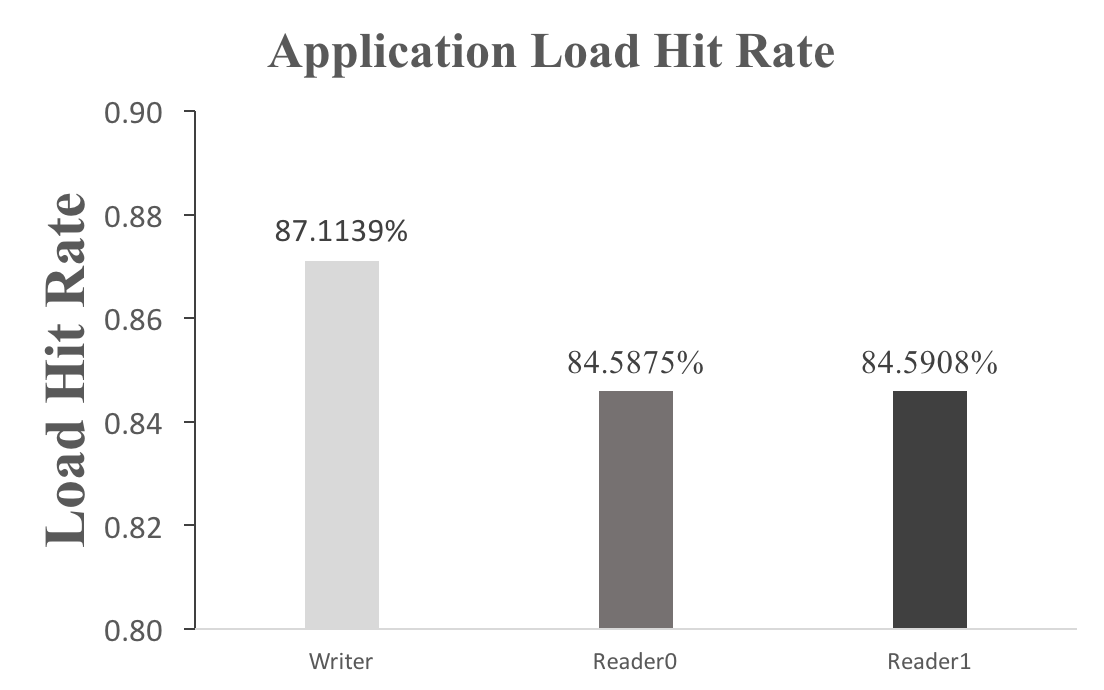
\includegraphics[width=3.5in]{write_invalidate.png}
\caption{Write-Invalidate Performance}
\label{write_invalidate}
\end{figure}
\FloatBarrier

\subsection{Write-Update Performance}
As Figure \ref{write_update} indicates, the entire program’s performance is good and for the shared data alone the load hit rate is perfect. This is because consumers get the data transferred from the produce and thus invalidation and memory reads are no longer needed.

\begin{figure}[!h]
\centering
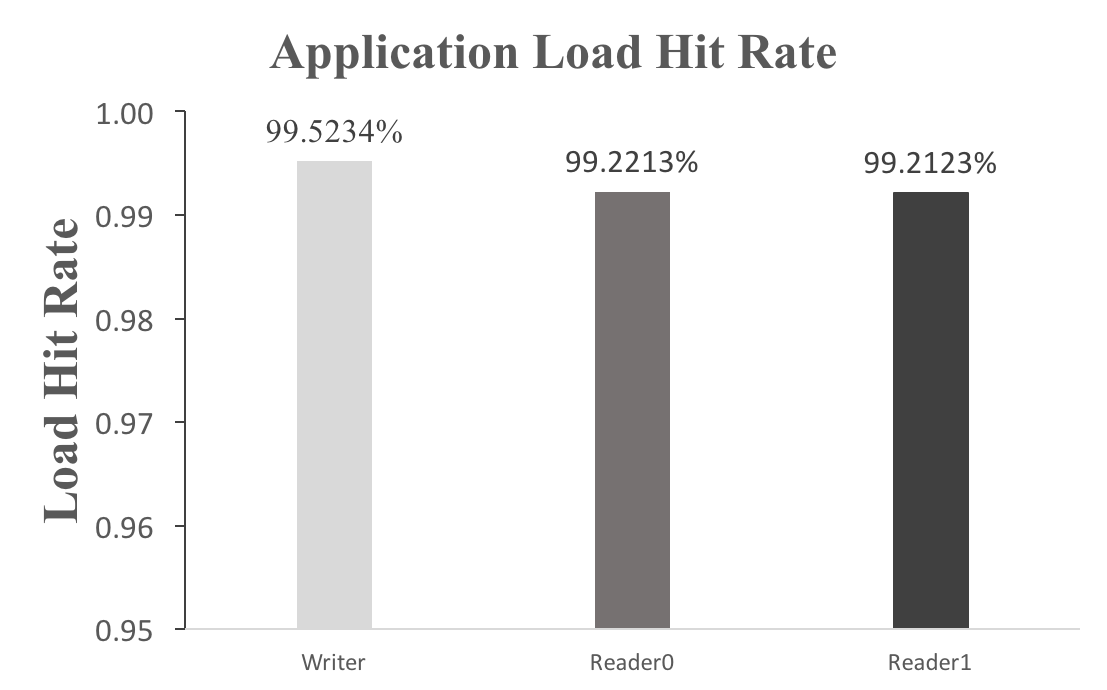
\includegraphics[width=3.5in]{write_update.png}
\caption{Write-Invalidate Performance}
\label{write_update}
\end{figure}
\FloatBarrier

\section{Adaptive Cache Coherence Protocol}
In this section, we introduce an adaptive cache coherence protocol that speculatively pushes data to consumers once producer-consumer patterns are detected. Extra bits are needed to track access history for each cache line. They are associated with directory lines which are extended to the structure shown in Figure \ref{dir_line}.

\begin{figure}[!h]
\centering
\captionsetup{justification=centering}
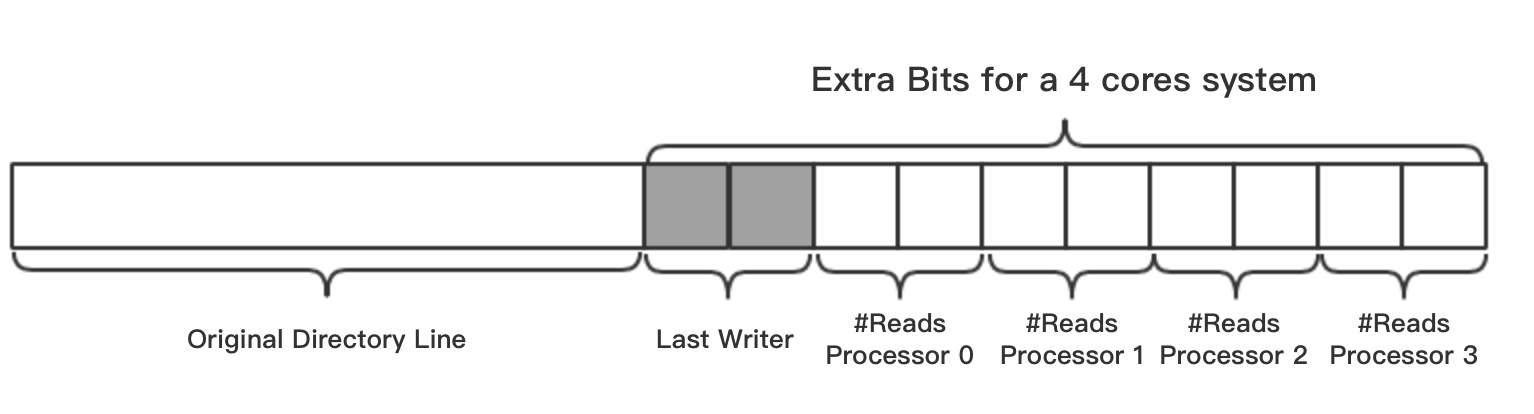
\includegraphics[width=3.5in]{dir_line.png}
\caption{Extended Directory Line Structure}
\label{dir_line}
\end{figure}
\FloatBarrier

The extra bits introduced for every cache line is
\begin{equation*}
log N + 2 * N
\end{equation*}
where $N$ is the number of processors, $last\_writer$ tracks the last one to write this cache line, and there are 2 saturating bits for every processor to track the number of read operations on this cache line. Cache accesses will trigger updates on the extra bits as shown in Algorithm \ref{write_operations} and \ref{read_operations}. Note that the extra bits will be discarded to save space when its associated directory line is evicted.

\begin{algorithm}
\caption{On Write Operations}
\label{write_operations}
\begin{algorithmic}[1]
\State Let $writer\_id$ be the processor performing writes
\If{$writer\_id$ == $last\_writer$}
    \ForAll{$pid \neq writer\_id$} \Comment{exclude itself}
        \If{CountReads($pid$) $>=$ 1}
            \State Cache2CacheDataPush($pid$) \Comment{write-update}
        \Else
            \State InvalidateDataCopy($pid$) \Comment{write-invalidate}
        \EndIf
        \State SaturatingDecrease($pid$) \Comment{decrease by 1}
    \EndFor
\Else
    \ForAll{$pid \neq writer\_id$} \Comment{exclude itself}
        \State InvalidateDataCopy($pid$) \Comment{write-invalidate}
        \State ClearCount($pid$) \Comment{reset read counts}
    \EndFor
    \State UpdateLastWriter($writer\_id$)
\EndIf
\end{algorithmic}
\end{algorithm}

\begin{algorithm}
\caption{On Read Operations}
\label{read_operations}
\begin{algorithmic}[1]
\State Let $pid$ refer to a processor
\ForAll{$pid$}
    \State SaturatingIncrease($pid$) \Comment{increase by 1}
\EndFor
\end{algorithmic}
\end{algorithm}



\section{Adaptive Protocol Evaluation}


\section{Summary}


\section{Future Works}


\newpage

\begin{thebibliography}{1}

\bibitem{ref1}
https://en.wikipedia.org/wiki/Producer-–consumer\_problem

\bibitem{ref2}
Cheng, Liqun, John B. Carter, and Donglai Dai. "An adaptive cache coherence protocol optimized for producer-consumer sharing." High Performance Computer Architecture, 2007. HPCA 2007. IEEE 13th International Symposium on. IEEE, 2007.

\end{thebibliography}

\end{document}
